\documentclass[10pt,a4paper]{article}

% Configuración de idioma y codificación
\usepackage[utf8]{inputenc}
\usepackage[spanish]{babel}

% Configuración de márgenes: Superior 5cm, Inferior 4cm, Izquierdo 4cm, Derecho 4cm 
\usepackage[top=5cm, bottom=4cm, left=4cm, right=4cm]{geometry}

% Tipografía base: Times New Roman 
\usepackage{times}

% Paquetes para figuras, tablas y matemáticas
\usepackage{graphicx}
\usepackage{amsmath}
\usepackage{caption}
\usepackage{multirow}
\usepackage{float}

% Configuración de los tamaños de los títulos de sección 
\usepackage{titlesec}
% Título de primer nivel: 14pt, Negrita
\titleformat{\section}{\normalfont\fontsize{14}{17}\bfseries}{\thesection}{1em}{}
% Título de segundo nivel: 12pt, Negrita
\titleformat{\subsection}{\normalfont\fontsize{12}{15}\bfseries}{\thesubsection}{1em}{}
% Título de tercer nivel: 10pt, Negrita
\titleformat{\subsubsection}{\normalfont\fontsize{10}{12}\bfseries}{\thesubsubsection}{1em}{}

% Configuración para código fuente: Courier New 10pt
\usepackage{listings}
\lstset{
    basicstyle=\fontsize{10}{12}\ttfamily,
    breaklines=true,
    frame=none,
    tabsize=4
}

% Paquete para pseudocódigo
\usepackage[ruled,vlined,linesnumbered,spanish]{algorithm2e}

% Ajuste para que las referencias bibliográficas se vean como [AutorAño]
\makeatletter
\renewcommand{\@biblabel}[1]{[#1]}
\makeatother

\begin{document}

% --- TÍTULO --- 
\begin{center}
    % Título del artículo: 16pt, Negrita
    \textbf{\fontsize{16}{19}\selectfont Predictor de la propagación de incendios}
\end{center}
\vspace{0.5cm}

% --- AUTORES Y FILIACIÓN --- 
\begin{center}
    % Autores: 12pt, Negrita
    \textbf{\fontsize{12}{15}\selectfont Renzo Dávila, Alejandro Moreno, Ramiro Martinez, Facundo Lella} \\
    % Filiación: 10pt, Normal
    \fontsize{10}{12}\selectfont Universidad Nacional de Cuyo, Facultad de Ingeniería \\
    Licenciatura en Ciencias de la Computación
\end{center}
\vspace{0.5cm}

% --- ABSTRACT Y KEYWORDS --- 
% Abstract en 10pt, Cursiva
\noindent \textit{\textbf{Abstract:} Este trabajo analiza conceptos de programación paralela y distribuida mediante la paralelización de un simulador de propagación de incendios forestales basado en autómatas celulares. Se desarrollaron una versión secuencial y una paralela con MPI, utilizando descomposición de dominio 2D, intercambio de halos y reducción colectiva. Se ejecutaron experimentos en un cluster variando el tamaño del problema, la cantidad de procesos y focos de incendio, y se analizaron métricas como speedup, eficiencia y overhead de comunicación, evaluando las métricas del algoritmo frente a distintas configuraciones.} \\

\vspace{0.2cm}
\noindent \textit{\textbf{Keywords:} Programación Paralela, MPI, Autómatas celulares}
\vspace{0.5cm}

% --- INTRODUCCIÓN --- 
\section{Introducción}
Este trabajo aborda la simulación de propagación de incendios forestales para analizar técnicas de computación paralela. El problema se modela como un autómata celular en una grilla 2D, representando un terreno generado proceduralmente (mediante ruido fractal) con cinco estados posibles: \textbf{Agua}, \textbf{Bosque}, \textbf{Ciudad}, \textbf{Quemándose} y \textbf{Ceniza}.

La propagación utiliza la vecindad de Von Neumann. Las celdas combustibles adyacentes al fuego se encienden según una probabilidad basada en su tipo de terreno y la dirección del viento. Para asegurar reproducibilidad independiente de la paralelización, la ignición emplea una función hash determinística pura basada en coordenadas.

La naturaleza del problema, donde cada celda depende solo de su vecindad inmediata, permite una fuerte paralelización mediante descomposición de dominio. Esto introduce desafíos algorítmicos como el intercambio de bordes (halos) y la coordinación global para detectar la extinción. El informe detalla la implementación secuencial, su paralelización con MPI y el análisis empírico de rendimiento en cluster.

% --- DESARROLLO ---
\section{Desarrollo}

\subsection{La simulación}
La simulación combina la generación procedural de un entorno y un motor de propagación basado en autómatas celulares.

\subsubsection{Autómatas celulares y Ruido fractal}
El modelo evoluciona en pasos de tiempo discretos usando la vecindad de Von Neumann [Wol83]. La grilla representa un terreno con cinco estados: \textbf{Agua}, \textbf{Bosque}, \textbf{Ciudad}, \textbf{Quemándose} y \textbf{Ceniza}. Para generar mapas visualmente realistas, el terreno se construye mediante ruido fractal [Per85] con múltiples \textit{octavas} [EMP+03], permitiendo definir lagos y zonas urbanas contiguas mediante umbrales y pasos de limpieza.

\subsubsection{Propagación y Frontera Activa}
El fuego inicia en focos aleatorios [Dur64] dictados por la semilla global. Para modelar la duración del fuego, su estado se gestiona en tres listas (\texttt{listaFuego1}, \texttt{listaFuego2}, \texttt{listaFuego3}). En cada iteración las celdas avanzan de lista hasta apagarse (Ceniza). 
Para optimizar el recorrido, se emplea el concepto de \textit{frontera activa}: solo se examinan los vecinos de celdas en llamas, reduciendo drásticamente la complejidad computacional. Una matriz booleana (o \texttt{unordered\_set} en paralelo) evita procesar celdas candidatas duplicadas.

\subsubsection{Probabilidades de ignición y efecto del viento}

La probabilidad de que una celda combustible se encienda depende de su tipo y de cuántos vecinos en llamas posee. La probabilidad base por vecino ardiente es del 42\% para Bosque y del 24\% para Ciudad. Cuando una celda tiene múltiples vecinos en llamas, se aplica un modelo de probabilidad acumulada basado en eventos independientes:

\begin{equation}
    P_{\text{ignición}} = 1 - \prod_{i=1}^{v} (1 - p_{\text{base}} \cdot w_{i})
\end{equation}

\noindent donde $v$ es la cantidad de vecinos en llamas y $w_{i}$ es el modificador de viento correspondiente al vecino $i$. El viento modifica la probabilidad de propagación de forma asimétrica según la dirección relativa entre la celda en llamas y la celda candidata:

\begin{table}[h]
\centering
\begin{tabular}{|l|c|}
\hline
\textbf{Dirección relativa} & \textbf{Modificador} \\ \hline
A favor del viento          & $\times 1.3$         \\ \hline
Perpendicular al viento     & $\times 0.7$         \\ \hline
Contra el viento            & $\times 0.3$         \\ \hline
\end{tabular}
\caption{Modificadores de probabilidad según la dirección del viento.}
\end{table}

\subsubsection{Decisión determinística de ignición}

Para garantizar que la versión secuencial y la paralela produzcan resultados idénticos con los mismos parámetros, la decisión de si una celda se enciende no utiliza un generador de números pseudoaleatorios con estado mutable. En su lugar, se emplea una función hash determinística basada en \textit{SplitMix64} [Ste14] que recibe como entrada la semilla global, el número de iteración y las coordenadas globales de la celda. Esto produce un valor uniformemente distribuido en $[0, 1)$ que se compara con la probabilidad de ignición calculada. Como la función depende únicamente de parámetros globales y no del orden de recorrido, el resultado es independiente de cómo se distribuya la grilla entre procesos MPI.

\subsection{Algoritmo secuencial}
La versión secuencial sirve como línea base de rendimiento y referencia de corrección. Opera en dos fases: generación del mapa y bucle de simulación iterativo.

\subsubsection{Flujo de la simulación}
En cada iteración del bucle principal ocurren los siguientes pasos:
\begin{enumerate}
    \item \textbf{Identificación}: Se recorren las celdas en llamas para obtener vecinos combustibles. Una matriz booleana filtra los duplicados.
    \item \textbf{Evaluación}: Cada candidato calcula su probabilidad acumulada (aplicando multiplicadores de viento) y se evalúa su ignición usando un hash determinístico basado en \textit{SplitMix64} [Ste14].
    \item \textbf{Transición}: Las listas rotan; las celdas apagadas pasan definitivamente al estado de Ceniza.
    \item \textbf{Terminación}: El bucle finaliza cuando no restan celdas activas en las listas.
\end{enumerate}

El Algoritmo \ref{alg:secuencial} ilustra una iteración secuencial.

\begin{algorithm}[H]
\caption{Iteración del algoritmo secuencial de propagación}\label{alg:secuencial}
\KwIn{Matriz $M$ de $n \times m$, listas $L_1, L_2, L_3$, semilla $s$, iteración $t$, viento $w$}
\KwOut{Listas actualizadas $L_1, L_2, L_3$}

$visitado \leftarrow$ matriz booleana $n \times m$ inicializada en \textbf{falso}\;
$candidatos \leftarrow$ lista vacía\;

\ForEach{celda $c$ en $L_1 \cup L_2 \cup L_3$}{
    \ForEach{vecino $v$ de $c$ (arriba, abajo, izquierda, derecha)}{
        \If{$M[v]$ es combustible \textbf{y} $visitado[v]$ es \textbf{falso}}{
            $visitado[v] \leftarrow$ \textbf{verdadero}\;
            agregar $v$ a $candidatos$\;
        }
    }
}

$nuevosFuegos \leftarrow$ lista vacía\;
\ForEach{celda $v$ en $candidatos$}{
    $p \leftarrow$ calcular probabilidad de ignición de $v$ con viento $w$\;
    $r \leftarrow$ hash determinístico$(s, t, v.fila, v.col)$\;
    \If{$r \leq p$}{
        agregar $v$ a $nuevosFuegos$\;
    }
}

\ForEach{celda $c$ en $L_3$}{
    $M[c] \leftarrow$ Ceniza\;
}

$L_3 \leftarrow L_2$\;
$L_2 \leftarrow L_1$\;
$L_1 \leftarrow nuevosFuegos$\;

\ForEach{celda $c$ en $L_1$}{
    $M[c] \leftarrow$ Quemándose\;
}
\end{algorithm}

\subsubsection{Decisiones de diseño}

Se tomaron varias decisiones orientadas a optimizar el rendimiento y facilitar la posterior paralelización:

\begin{itemize}
    \item \textbf{Frontera activa en lugar de barrido completo}: recorrer solo los vecinos de las celdas en llamas reduce la complejidad por iteración de $O(n \times m)$ a $O(k)$, donde $k$ es el tamaño de la frontera. En matrices de $10000 \times 10000$ o mayores, esta optimización resulta fundamental.
    \item \textbf{Deduplicación con matriz booleana}: se optó por una matriz de booleanos ($n \times m$) en lugar de una tabla hash de coordenadas. Si bien ambas opciones evitan evaluar candidatos duplicados, la matriz booleana ofrece acceso $O(1)$ con mejor localidad de caché, al costo de una mayor huella de memoria. Esta decisión se invierte en la versión paralela, donde cada proceso maneja un bloque más pequeño y la reconstrucción de una matriz completa sería innecesaria.
    \item \textbf{Listas contiguas en memoria}: las tres listas de fuego se implementan como arreglos dinámicos contiguos, lo que permite iteración eficiente y transferencia entre listas mediante movimiento de punteros sin copia de datos.
    \item \textbf{Hash determinístico sin estado}: el uso de una función hash pura en lugar de un generador pseudoaleatorio con estado mutable fue una decisión orientada a la paralelización. Al no depender del orden de evaluación de los candidatos, la misma función puede utilizarse en la versión paralela sin requerir sincronización del estado aleatorio entre procesos.
    \item \textbf{Separación de módulos}: la generación del entorno y el algoritmo de propagación se mantienen en módulos independientes. Esto permite que la versión paralela reutilice el mismo generador de entornos, garantizando que ambas versiones operen sobre mapas idénticos dada la misma semilla.
\end{itemize}

\subsection{Algoritmo paralelo}
El paralelismo se basa en el particionamiento de datos espaciales. Cada evaluación celular depende solo de la vecindad ortogonal inmediata. Se sigue un modelo SPMD (\textit{Single Program, Multiple Data}) y la asignación es estática por simplicidad. Las fases de generación del entorno y recolección final del mapa operan secuencialmente en el proceso raíz.

\subsubsection{Descomposición de dominio}
La matriz se particiona en bloques cartesianos 2D contiguos usando \texttt{MPI\_Dims\_create()} y \texttt{MPI\_Cart\_create()}. Los sobrantes dimensionales se distribuyen entre los primeros rangos. Cada proceso maneja su submatriz y una frontera de una celda (\textit{halo}) en cada dirección ortogonal. Al utilizar \texttt{MPI\_Cart\_shift()}, los vecinos fuera de los bordes del mapa resuelven en \texttt{MPI\_PROC\_NULL}, evitando lógica condicional periférica.

\subsubsection{Flujo de iteración e Implementación MPI}
En cada iteración, los procesos ejecutan simétricamente:
\begin{enumerate}
    \item \textbf{Intercambio de halos}: Las fronteras se transfieren a los vecinos mediante llamadas bloqueantes punto a punto (\texttt{MPI\_Sendrecv}), evadiendo interbloqueos.
    \item \textbf{Identificación}: Se evalúan las celdas ardientes locales y las reportadas como \textit{Quemándose} dentro de los halos recibidos. Un \texttt{unordered\_set} deduplica candidatos, minimizando la huella de memoria.
    \item \textbf{Evaluación y Transición}: Similar al algoritmo secuencial.
    \item \textbf{Sincronización global}: Mediante la primitiva colectiva \texttt{MPI\_Allreduce} (operación \texttt{MPI\_SUM}), se totalizan los fuegos activos de todos los nodos. Si el resultado global es nulo, la simulación concluye.
\end{enumerate}

Para la distribución inicial de parámetros y sub-matrices se emplean \texttt{MPI\_Bcast} y flujos punto a punto repetidos (\texttt{MPI\_Send}/\texttt{MPI\_Recv}). La memoria interna utiliza almacenamiento contiguo unidimensional (\texttt{std::vector}) para maximizar la localidad de caché. El Algoritmo \ref{alg:paralelo} resume la lógica distribuida.

\subsection{Parámetros y Ejecución}
El sistema se compiló utilizando el estándar C++17, \texttt{g++} y OpenMPI 4.1.4. Se dispone de \textit{targets} de Makefile adaptados tanto para compilación con renderizado gráfico SDL2 como para clusters (deshabilitando la interfaz gráfica).

Ambas versiones comparten una interfaz CLI basada en banderas de línea de comando (\texttt{--rows}, \texttt{--cols}, \texttt{--iterations}, \texttt{--fires}, \texttt{--seed}, y \texttt{--wind}). La ejecución paralela se inicializa mediante el lanzador MPI (por ejemplo, \texttt{mpirun -np 8 ./mpi\_fire}). Las pruebas en cluster se despacharon utilizando el gestor de recursos SLURM para centralizar y aislar las métricas computacionales.

% --- ESTUDIO EXPERIMENTAL ---
\section{Estudio experimental}

Para evaluar el rendimiento del programa y analizar el impacto de la paralelización frente a distintos escenarios, se elaboró un estudio empírico exhaustivo. Este proceso se divide en tres partes fundamentales: el diseño de las configuraciones a probar, la identificación de los factores que pueden afectar los tiempos de ejecución y la definición de las métricas de rendimiento a recolectar.

\subsection{Diseño de los experimentos}

En esta sección se detalla el conjunto de diferentes configuraciones tenidas en cuenta para realizar la experimentación. Se fijó la semilla del generador procedimental de mapas y decisiones de ignición en un valor constante (\texttt{seed = 67}), un límite máximo de 100\,000 iteraciones y sin direccion del viento. Se variaron los siguientes tres parámetros, explorando todas sus combinaciones posibles:

\begin{table}[h]
\centering
\begin{tabular}{|l|l|}
\hline
\textbf{Parámetro} & \textbf{Valores evaluados} \\ \hline
Tamaño de la matriz & $10000^2$, $15000^2$ y $20000^2$ celdas \\ \hline
Procesos MPI ($P$) & 1 (secuencial), 2, 4 y 8 \\ \hline
Focos iniciales & 1, 3 y 5 \\ \hline
\end{tabular}
\caption{Espacio de parámetros explorado en los experimentos.}
\end{table}

El cruce de estas tres variables arroja un total de $3 \times 4 \times 3 = 36$ configuraciones experimentales. Al fijar la semilla en 67, se garantiza que para un tamaño de matriz y cantidad de focos dados, tanto la versión secuencial como todas las versiones paralelas trabajen sobre exactamente el mismo mapa, posición de los focos y secuencia pseudoaleatoria de probabilidades de ignición.

\subsection{Factores que influyen en los resultados}

El tiempo de ejecución de cada simulación puede verse afectado significativamente por distintos factores tanto del algoritmo como del entorno físico en el cluster:

\begin{itemize}
    \item \textbf{Tamaño de la grilla frente al número de procesos:} A medida que se incrementa el número de procesos para una matriz de tamaño fijo, la porción de datos procesada localmente disminuye, pero la cantidad de comunicaciones (intercambio de halos y reducciones) se mantiene o aumenta, pudiendo ocasionar que el \textit{overhead} de comunicación eclipse la ganancia en poder de cómputo.
    \item \textbf{Ubicación y cantidad de los focos iniciales:} Dado que en esta experimentación no se aplica una dirección de viento preferencial, el fuego se propaga radialmente (de forma isotrópica) desde cada punto de ignición. Al añadir una mayor cantidad de focos (1, 3 y 5) distribuidos en el mapa, el terreno se consume desde múltiples frentes en simultáneo. Esto acelera el consumo del material combustible, provocando que la cantidad total de iteraciones necesarias para extinguir el incendio disminuya a medida que se aumentan los focos iniciales.
    \item \textbf{Overhead de comunicaciones y sincronización:} La primitiva \texttt{MPI\_Sendrecv} obliga a los procesos a esperarse mutuamente en cada iteración. Desequilibrios menores en el tamaño de la frontera del incendio en cada bloque pueden causar que un proceso deba esperar a su vecino, penalizando el tiempo global reportado.
    \item \textbf{Topología del cluster:} Si los procesos se ubican dentro de un mismo nodo físico utilizando memoria compartida, el paso de mensajes será considerablemente más rápido en comparación a ejecutar procesos comunicados a través de la red de interconexión entre distintos nodos del cluster.
\end{itemize}

\subsection{Métricas a obtener}

Para cuantificar el desempeño y comprender cómo responde el algoritmo al escalado paralelo, se registran y analizan las siguientes métricas:

\begin{itemize}
    \item \textbf{Tiempo de ejecución ($T$):} Representa el tiempo de pared (\textit{wall-clock time}) medido exclusivamente sobre el bucle de propagación de la simulación, descartando tiempos de inicialización de MPI, generación fractal del entorno y finalización, usando \texttt{MPI\_Wtime()}.
    \item \textbf{Iteración de extinción:} Instante discreto de tiempo en el que la simulación finaliza por la ausencia de fuego activo en toda la grilla. Es fundamental para verificar la correctitud algorítmica: todas las versiones (secuencial, 2, 4, 8 procesos) de un mismo tamaño de matriz y cantidad de focos deben detenerse exactamente en la misma iteración.
    \item \textbf{Speedup ($S$):} Indica el factor de aceleración introducido por el paralelismo. Se calcula como la relación entre el tiempo del caso secuencial y el caso paralelo para $p$ procesos, es decir, $S(p) = T(1) / T(p)$. Un speedup lineal sería lo ideal ($S(p) = p$).
    \item \textbf{Eficiencia ($E$):} Representa la fracción de tiempo que los procesos se mantienen realizando trabajo útil y se calcula como $E(p) = S(p) / p$. Valores cercanos a $1.0$ (o 100\%) indican un aprovechamiento óptimo de los núcleos computacionales involucrados.
\end{itemize}

\section{Resultados obtenidos}

En esta sección se presentan todos los resultados brutos obtenidos a partir de la ejecución de las configuraciones definidas en el diseño experimental. La Tabla \ref{tab:resultados_brutos} resume los tiempos de ejecución de la simulación medidos empíricamente en el cluster, expresados en milisegundos, así como la cantidad exacta de iteraciones que tomó extinguir cada incendio. Adicionalmente, la Tabla \ref{tab:metricas_profiling} expone un desglose detallado del tiempo consumido internamente por iteración para un caso de estudio específico ($10000^2$ con 8 procesos y 1 foco), diferenciando el cómputo local de los tiempos de comunicación. Por último, la Tabla \ref{tab:comparativa_focos} presenta una comparativa empírica de los costos de iteración al variar la cantidad de focos iniciales de 1 a 5, evidenciando el aumento de la carga computacional y de sincronización.

\begin{table}[h]
\centering
\begin{tabular}{|c|c|c|r|r|r|r|}
\hline
\multirow{2}{*}{\textbf{Matriz}} & \multirow{2}{*}{\textbf{Focos}} & \multirow{2}{*}{\textbf{Iteraciones}} & \multicolumn{4}{c|}{\textbf{Tiempo de ejecución (ms)}} \\ \cline{4-7}
 & & & \textbf{Secuencial} & \textbf{2 procesos} & \textbf{4 procesos} & \textbf{8 procesos} \\ \hline
\multirow{3}{*}{$10000^2$} & 1 & 15033 & 104148 & 26546.8 & 21063.0 & 17699.6 \\ \cline{2-7}
 & 3 & 12455 & 100334 & 37569.8 & 23231.2 & 19049.6 \\ \cline{2-7}
 & 5 & 11505 & 99656 & 36815.8 & 22877.8 & 18010.1 \\ \hline
\multirow{3}{*}{$15000^2$} & 1 & 26906 & 308017 & 62023.2 & 55405.2 & 37826.9 \\ \cline{2-7}
 & 3 & 25497 & 279798 & 87297.7 & 70329.0 & 47708.9 \\ \cline{2-7}
 & 5 & 23453 & 269076 & 89026.9 & 67654.3 & 46483.8 \\ \hline
\multirow{3}{*}{$20000^2$} & 1 & 30102 & 741801 & 109684.0 & 90247.6 & 71385.0 \\ \cline{2-7}
 & 3 & 24184 & 676599 & 145972.0 & 103823.0 & 79533.5 \\ \cline{2-7}
 & 5 & 23814 & 664370 & 145548.0 & 101118.0 & 78787.3 \\ \hline
\end{tabular}
\caption{Resultados empíricos de los tiempos de ejecución medidos en el cluster.}
\label{tab:resultados_brutos}
\end{table}

\begin{table}[h]
\centering
\begin{tabular}{|c|c|c|c|c|c|}
\hline
\textbf{Rank} & \textbf{Promedio de} & \textbf{Cómputo} & \textbf{Halos} & \textbf{Sincronización} & \textbf{Iteración} \\
\textbf{MPI} & \textbf{Candidatos} & \textbf{Útil (ms)} & \textbf{(ms)} & \textbf{MPI\_Allreduce (ms)} & \textbf{Total (ms)} \\ \hline
0 & 1530 & 0.318 & 0.051 & 0.747 & 1.173 \\
1 & 1560 & 0.327 & 0.052 & 0.736 & 1.173 \\
2 & 1395 & 0.298 & 0.058 & 0.764 & 1.173 \\
3 & 1865 & 0.376 & 0.058 & 0.671 & 1.173 \\
4 & 1439 & 0.303 & 0.067 & 0.750 & 1.173 \\
5 & 1126 & 0.253 & 0.067 & 0.810 & 1.173 \\
6 & 1789 & 0.356 & 0.070 & 0.683 & 1.173 \\
7 & 1541 & 0.322 & 0.070 & 0.724 & 1.173 \\ \hline
\end{tabular}
\caption{Desglose del tiempo promedio por iteración por proceso (Matriz $10000^2$, P=8, 1 Foco).}
\label{tab:metricas_profiling}
\end{table}

\begin{table}[H]
\centering
\begin{tabular}{|l|c|c|c|}
\hline
\textbf{Métrica Promedio (P=8)} & \textbf{1 Foco} & \textbf{5 Focos} & \textbf{Variación} \\ \hline
Iteraciones Totales & 15033 & 11505 & -23.4\% \\ \hline
Candidatos Máximos por Nodo & 1865 & 2437 & +30.6\% \\ \hline
Cómputo Útil Promedio (ms) & $\sim0.31$ & $\sim0.41$ & +32.2\% \\ \hline
Sincronización \texttt{MPI\_Allreduce} (ms) & $\sim0.74$ & $\sim1.01$ & +36.4\% \\ \hline
Tiempo Promedio por Iteración (ms) & 1.173 & 1.551 & +32.2\% \\ \hline
\end{tabular}
\caption{Comparativa del impacto en la carga de procesamiento al variar la cantidad de focos iniciales.}
\label{tab:comparativa_focos}
\end{table}
\space
\section{Análisis de los resultados}

A partir de los tiempos recolectados, se evalúa detalladamente el rendimiento y la ganancia computacional obtenida gracias a la paralelización del modelo mediante MPI. Se estudiaron las métricas derivadas para comprender el comportamiento de la arquitectura frente a una simulación con un uso intensivo de la memoria.

\subsection{Tiempo de ejecución (Rendimiento)}
Se observa una drástica reducción en los tiempos de ejecución al incorporar procesos paralelos. En la Figura \ref{fig:rendimiento} se presentan los gráficos de rendimiento para los tres tamaños de matriz. Destaca fuertemente la matriz de $20000^2$, donde la ejecución secuencial con un foco superó los 12 minutos (741 segundos), mientras que la versión paralela con 8 procesos completó la misma tarea en poco más de un minuto (71 segundos). 

Por otra parte, se evidencia un comportamiento asimétrico muy interesante al variar la cantidad de focos iniciales. En el caso secuencial, aumentar la cantidad de focos (de 1 a 5) reduce el tiempo total, dado que el mapa se consume rápidamente desde múltiples frentes y se requiere una menor cantidad de iteraciones. Sin embargo, en las ejecuciones paralelas sucede lo contrario: el tiempo total \textbf{aumenta}. 

Los datos de \textit{profiling} (Tabla \ref{tab:comparativa_focos}) lo justifican matemáticamente: al comparar la matriz de $10000^2$ con $P=8$, la simulación con 1 foco requiere 15033 iteraciones a un costo de $1.173$ ms por iteración. Al iniciar con 5 focos, el fuego activo irrumpe desde múltiples bloques MPI simultáneamente. Esto eleva dramáticamente el promedio de candidatos a evaluar por iteración (pasando de un máximo de 1865 a 2437 candidatos por nodo), incrementando la carga de cómputo útil y empeorando el cuello de botella de la sincronización. Como resultado empírico, aunque la simulación con 5 focos finaliza en menos ciclos (11505 iteraciones), el tiempo promedio que cuesta cada iteración individual se dispara un 32\% (pasando a $1.551$ ms), lo cual anula por completo el ahorro de iteraciones y resulta en un tiempo de reloj total más alto.

\begin{figure}[h]
    \centering
    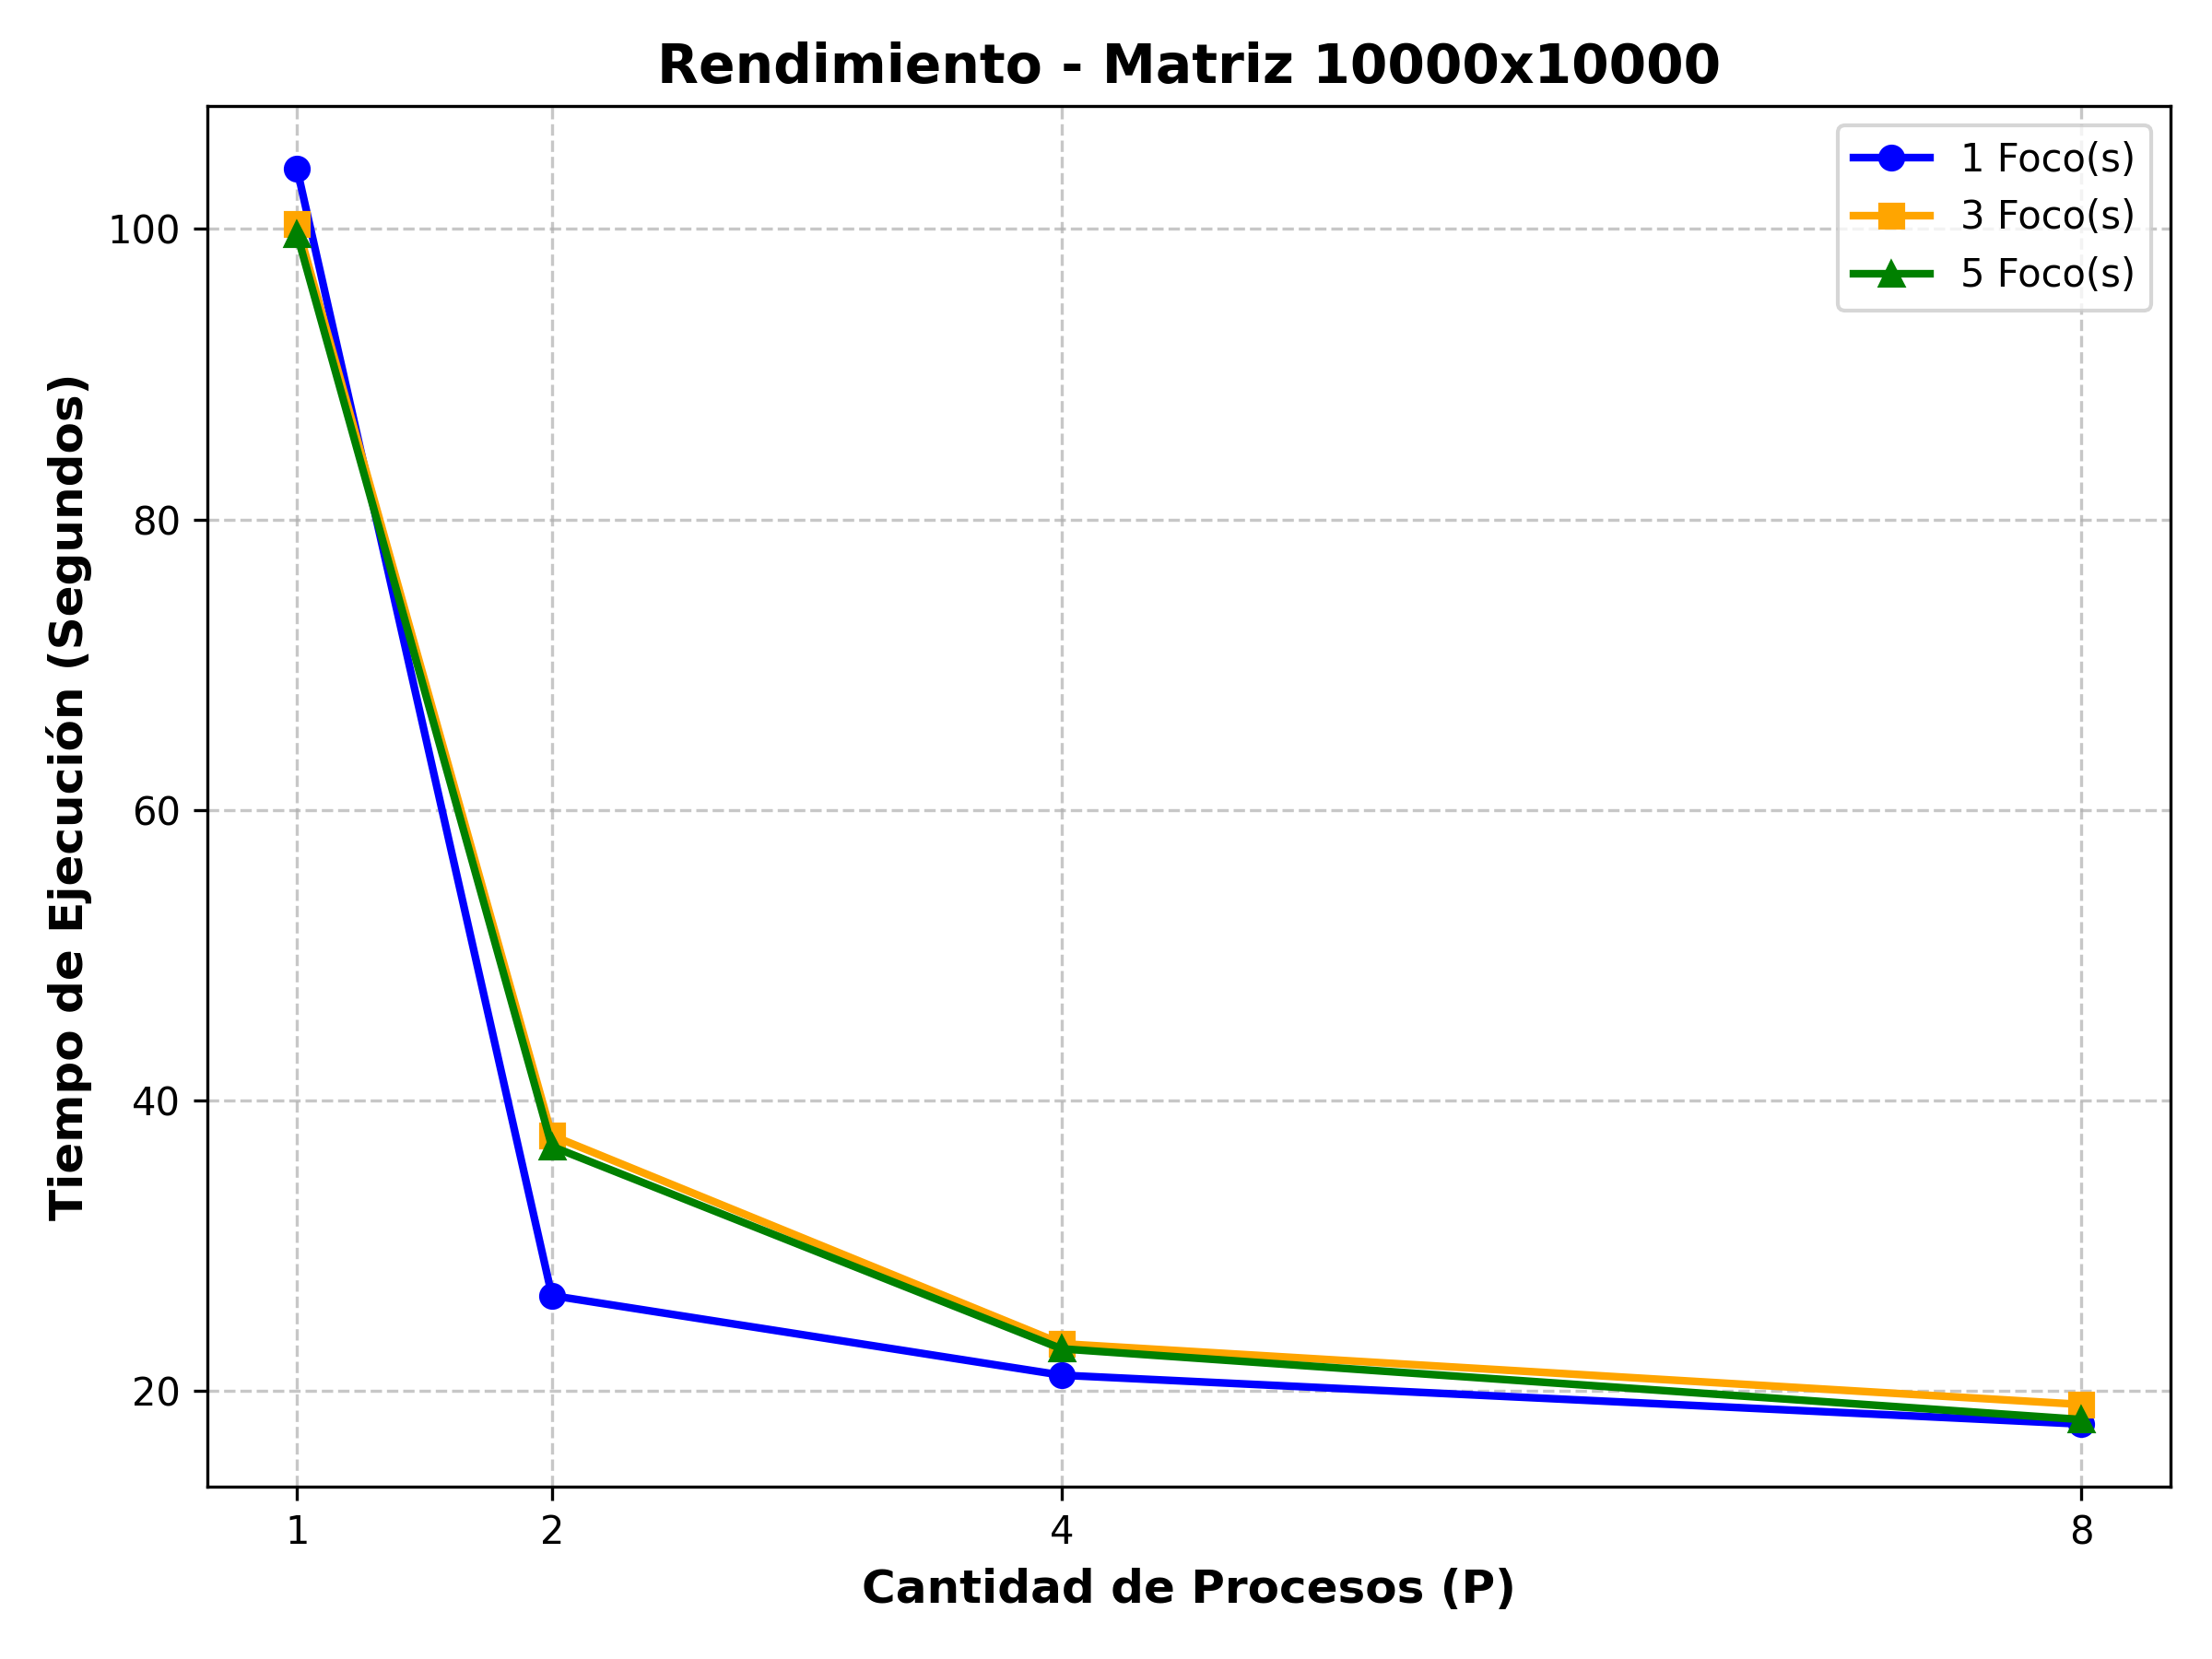
\includegraphics[width=0.32\textwidth]{graficos/rendimiento_10000x10000.png}
    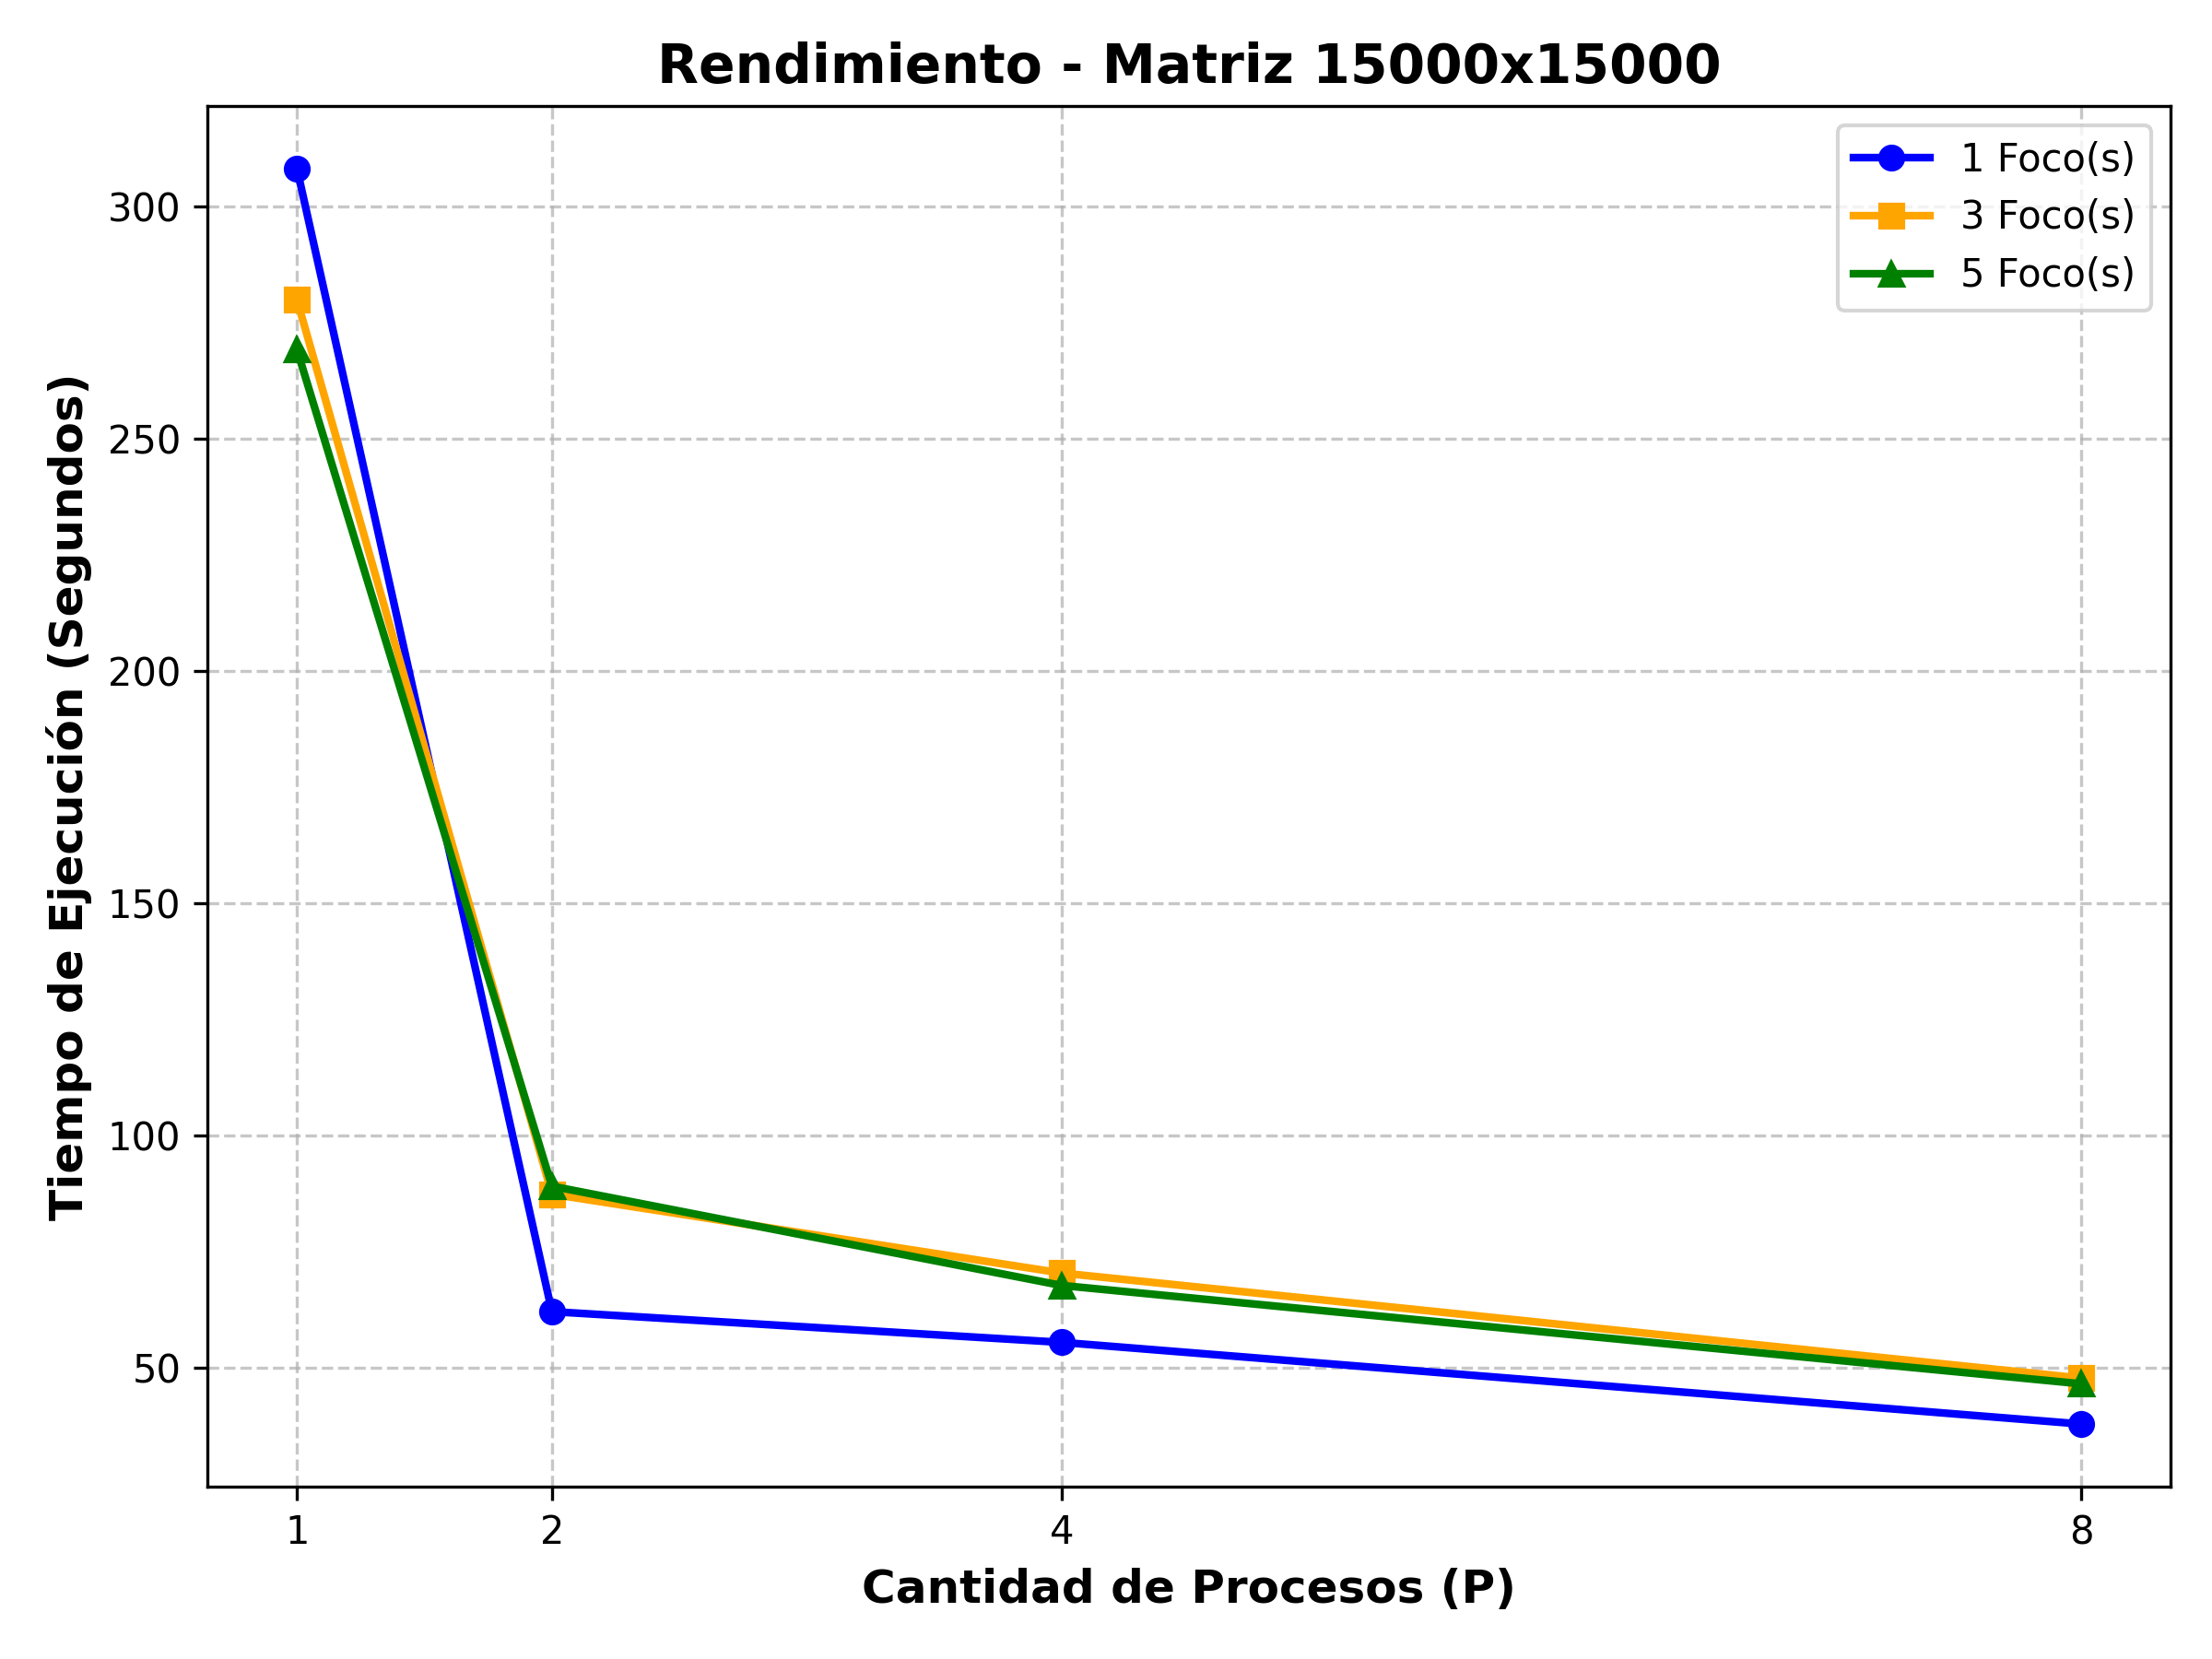
\includegraphics[width=0.32\textwidth]{graficos/rendimiento_15000x15000.png}
    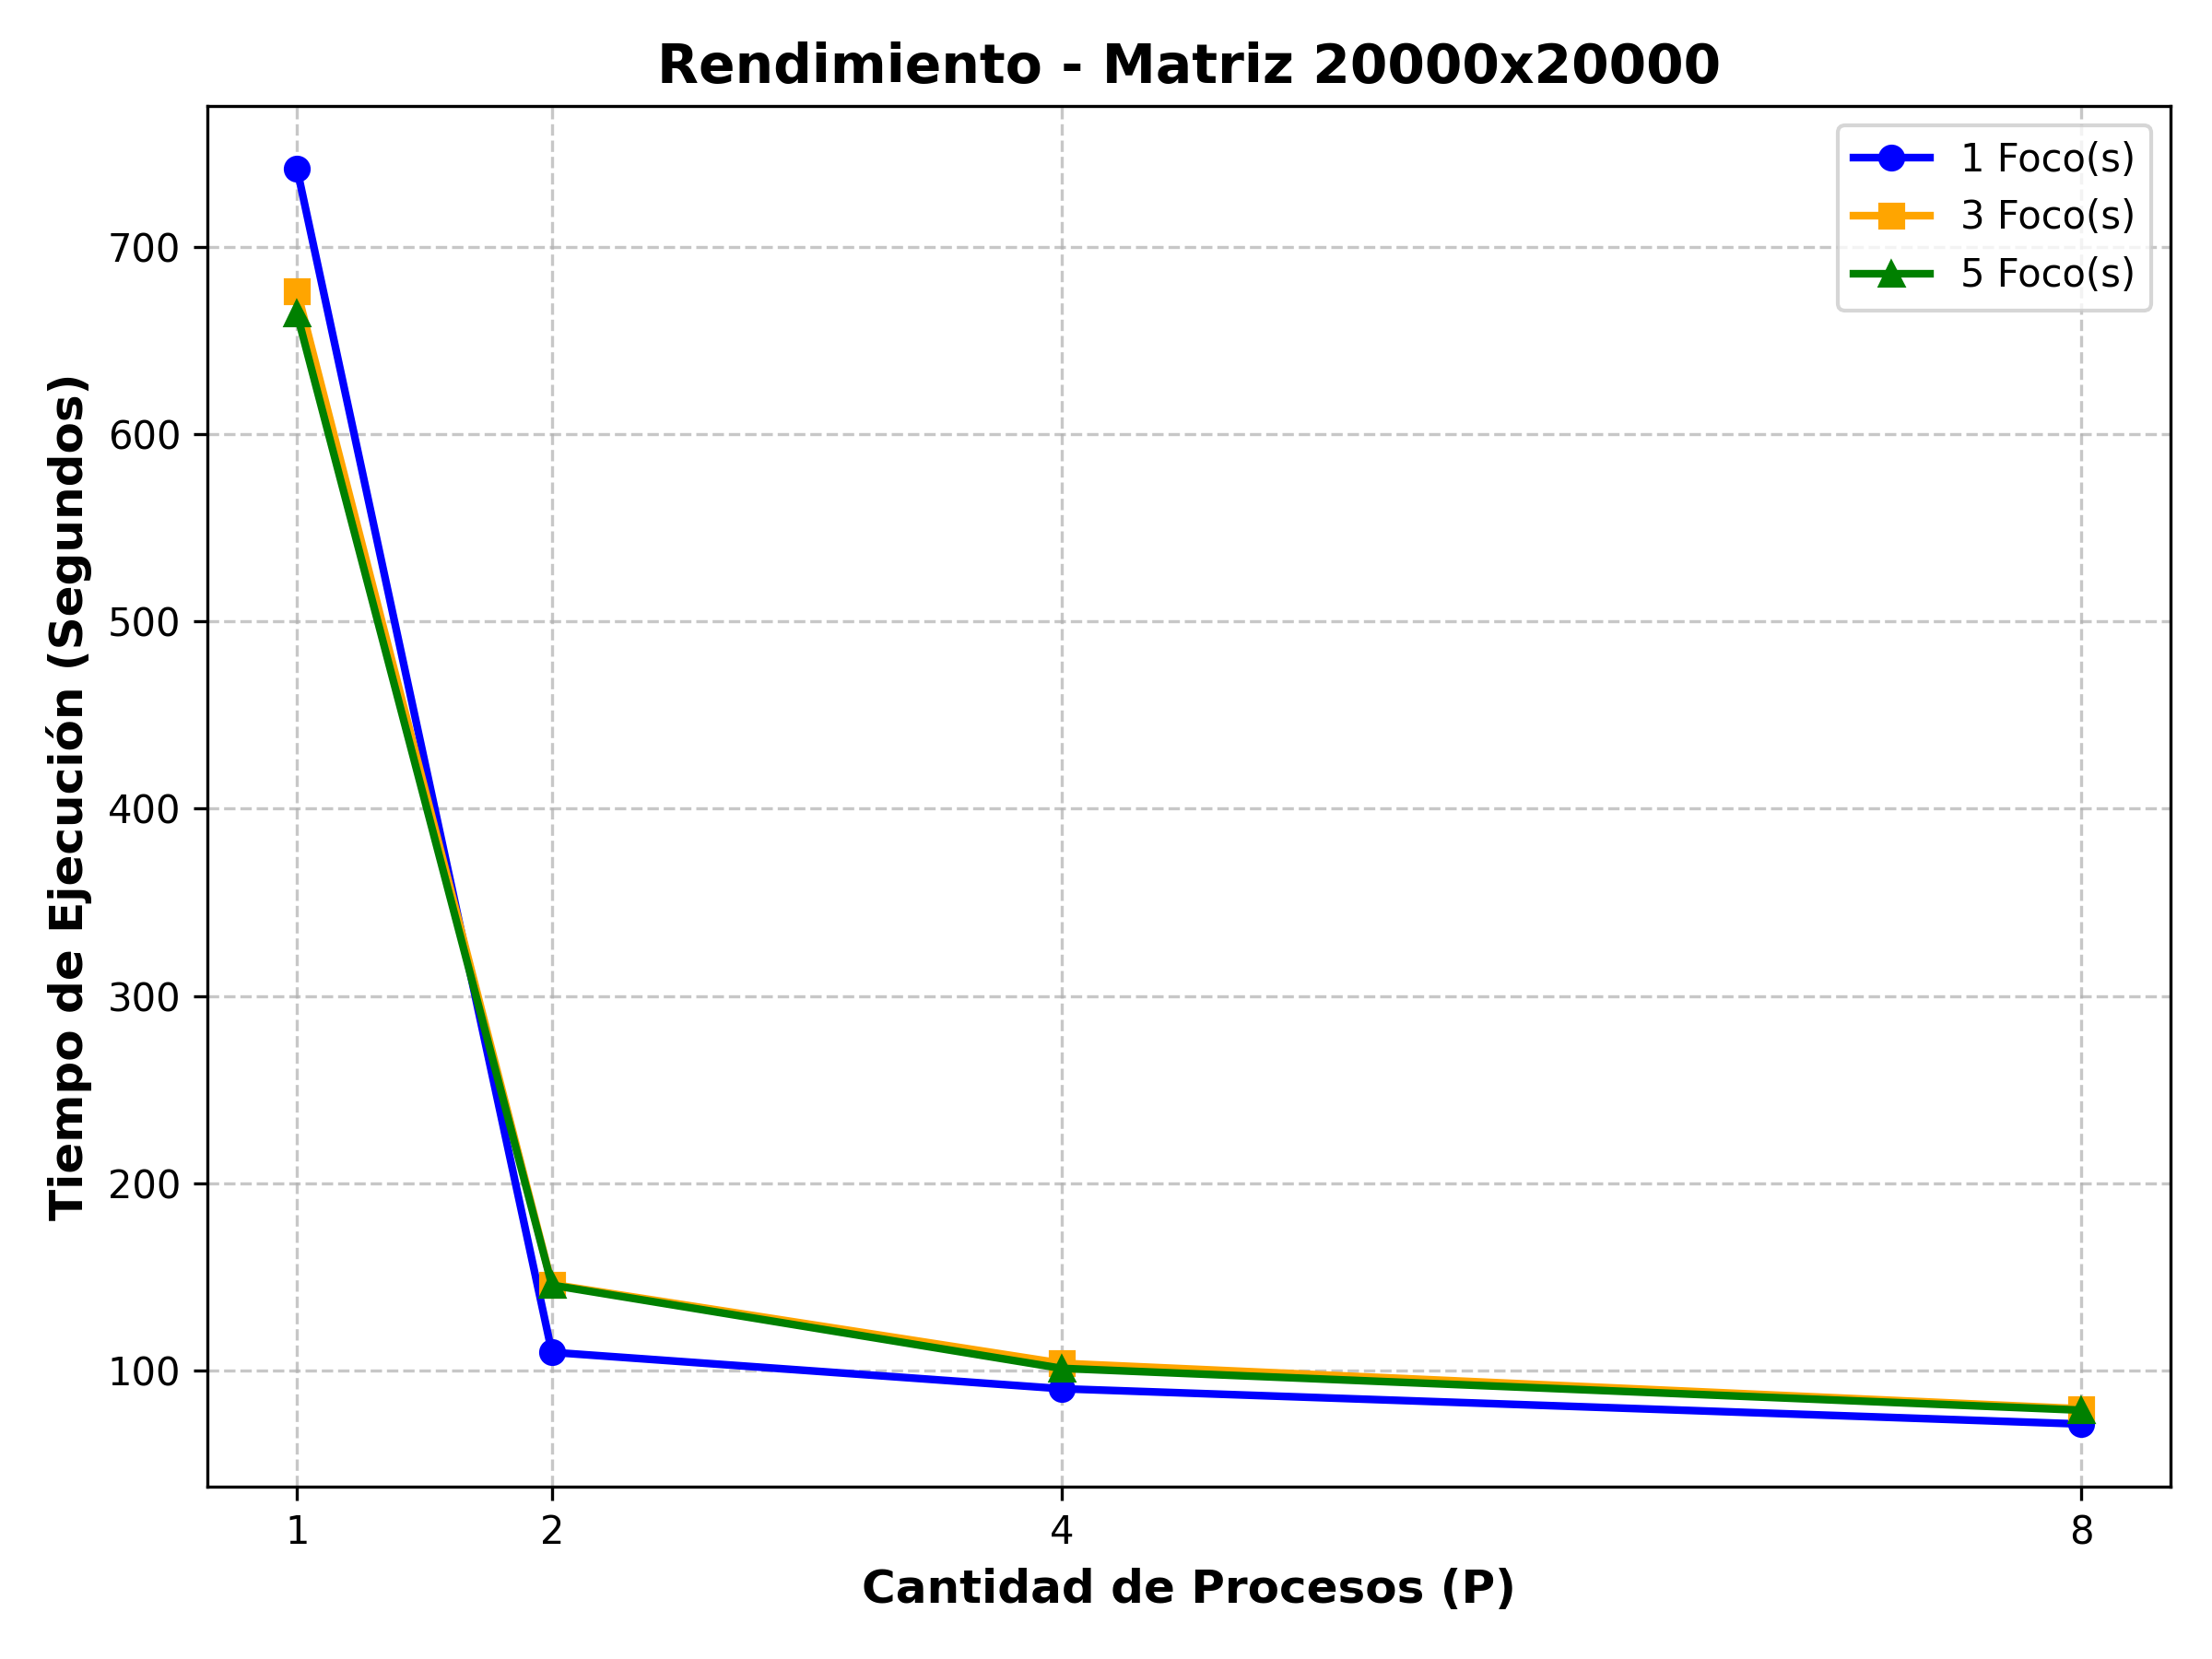
\includegraphics[width=0.32\textwidth]{graficos/rendimiento_20000x20000.png}
    \caption{Tiempos de ejecución (Rendimiento) en función de la cantidad de procesos MPI para grillas de $10000^2$, $15000^2$ y $20000^2$.}
    \label{fig:rendimiento}
\end{figure}

\subsection{Speedup y Aceleración Superlineal}
Al analizar el Speedup ($S = T_1 / T_p$), se evidencia un fenómeno excepcional conocido en la computación paralela como \textbf{Speedup Superlineal} ($S > p$). Como se observa en la Figura \ref{fig:speedup}, la aceleración lograda supera consistentemente el límite teórico ideal. Por ejemplo, en la matriz de $20000^2$ con 1 foco, el uso de 8 procesos logró un speedup de $10.4\times$.

Este fenómeno obedece a la arquitectura de memoria jerárquica del hardware. La matriz global de $20000^2$ requiere alojar 400 millones de enteros, lo cual excede por un amplio margen las memorias caché L2 y L3 de un único procesador, provocando constantes fallos de caché (\textit{cache misses}) en la versión secuencial. Al particionar el dominio mediante MPI, cada proceso local maneja bloques sustancialmente menores que caben de manera más eficiente en la memoria caché de su nodo. La enorme reducción en los tiempos de acceso a memoria es tan drástica que eclipsa con creces el costo computacional extra que supone intercambiar las fronteras (halos) por la red.

\begin{figure}[h]
    \centering
    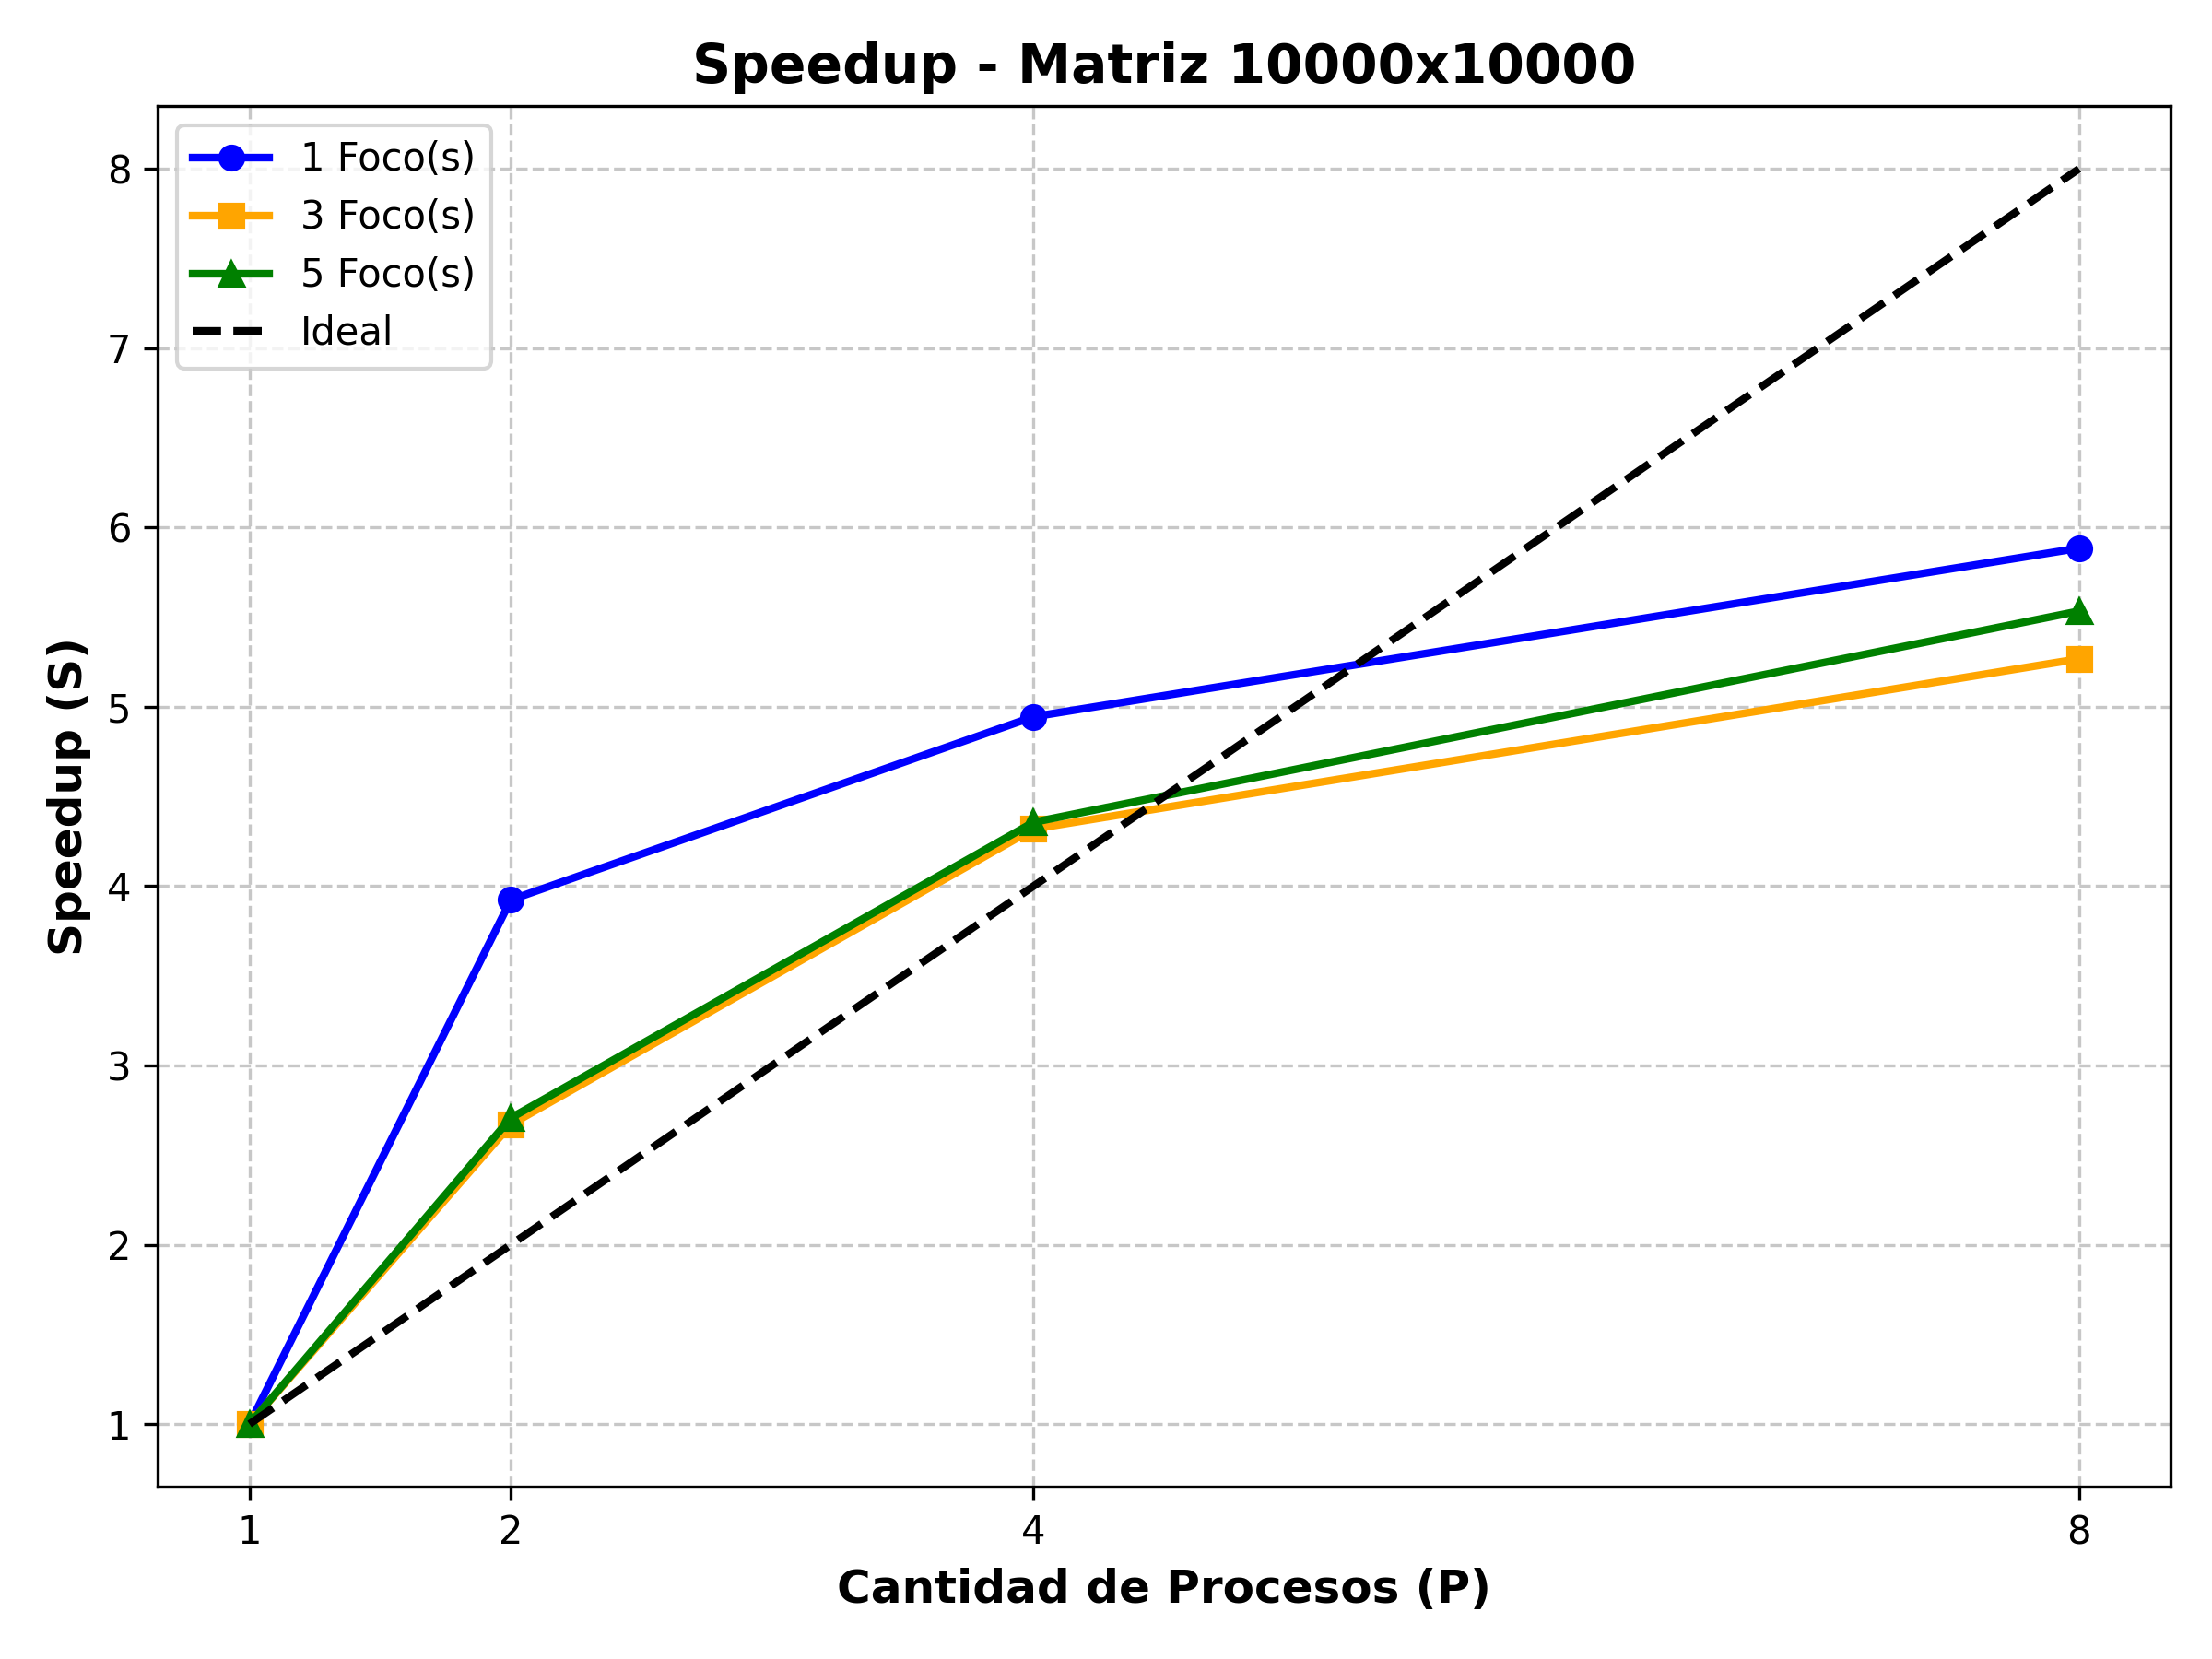
\includegraphics[width=0.32\textwidth]{graficos/speedup_10000x10000.png}
    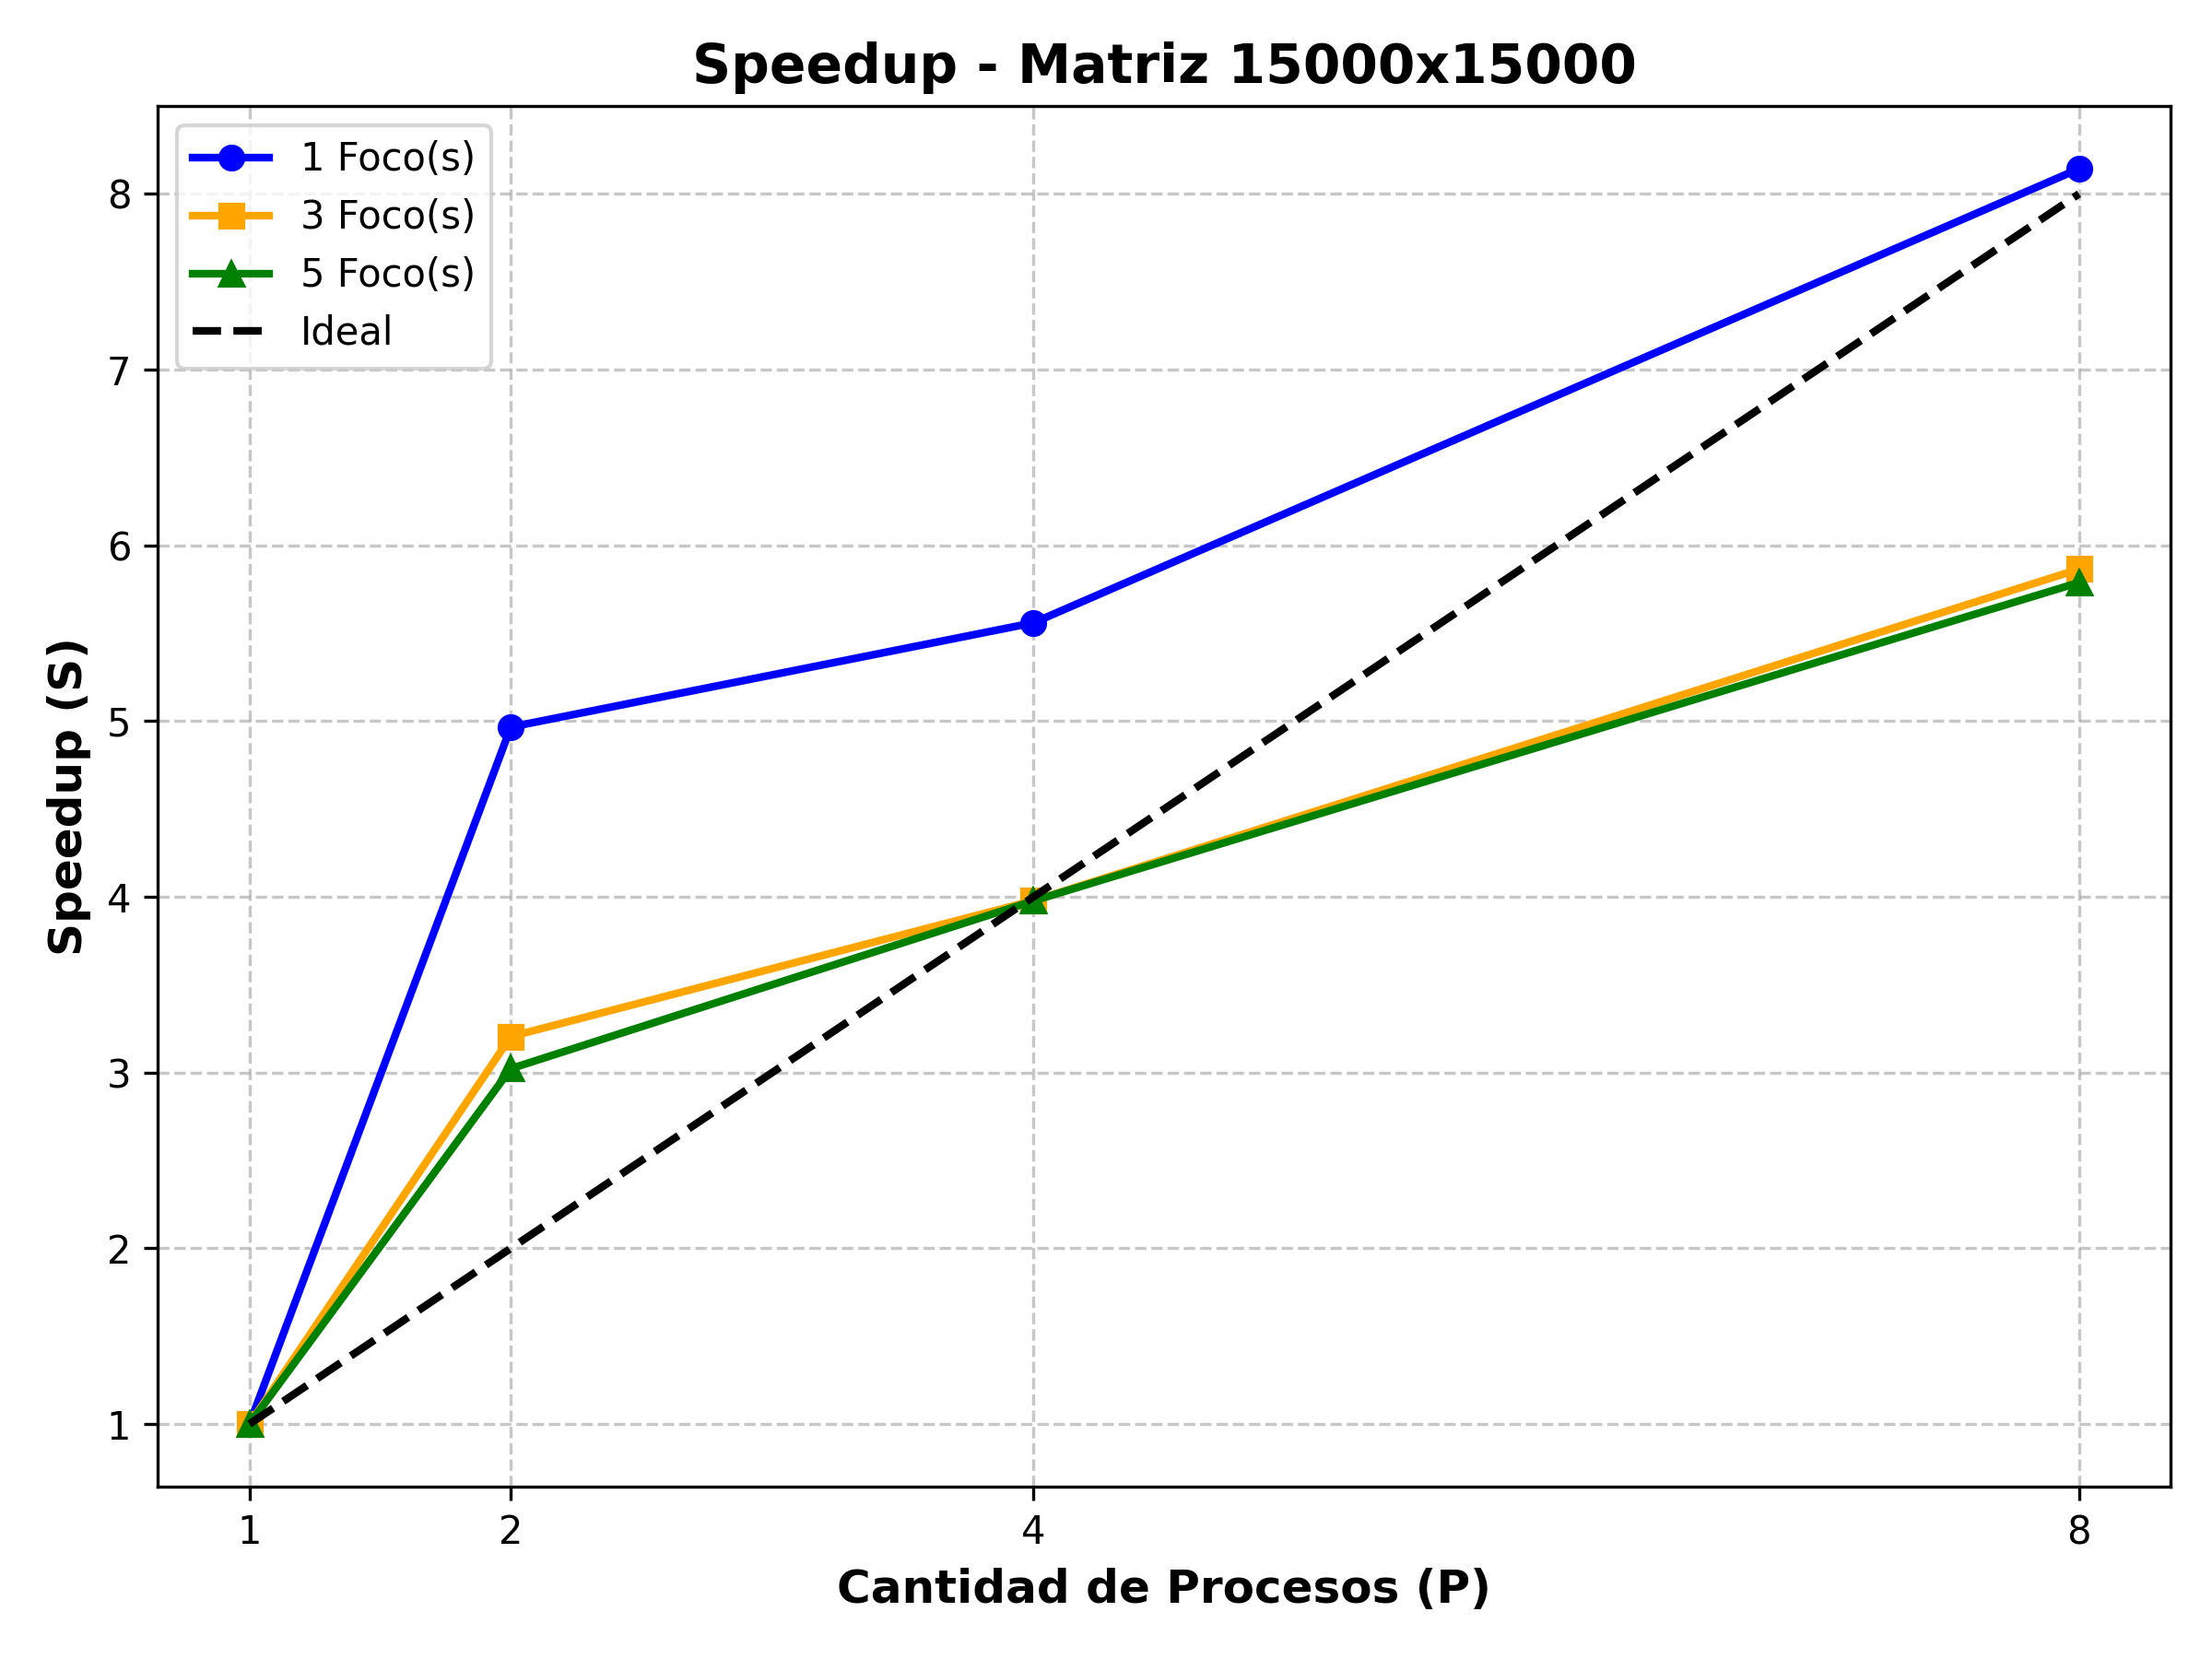
\includegraphics[width=0.32\textwidth]{graficos/speedup_15000x15000.png}
    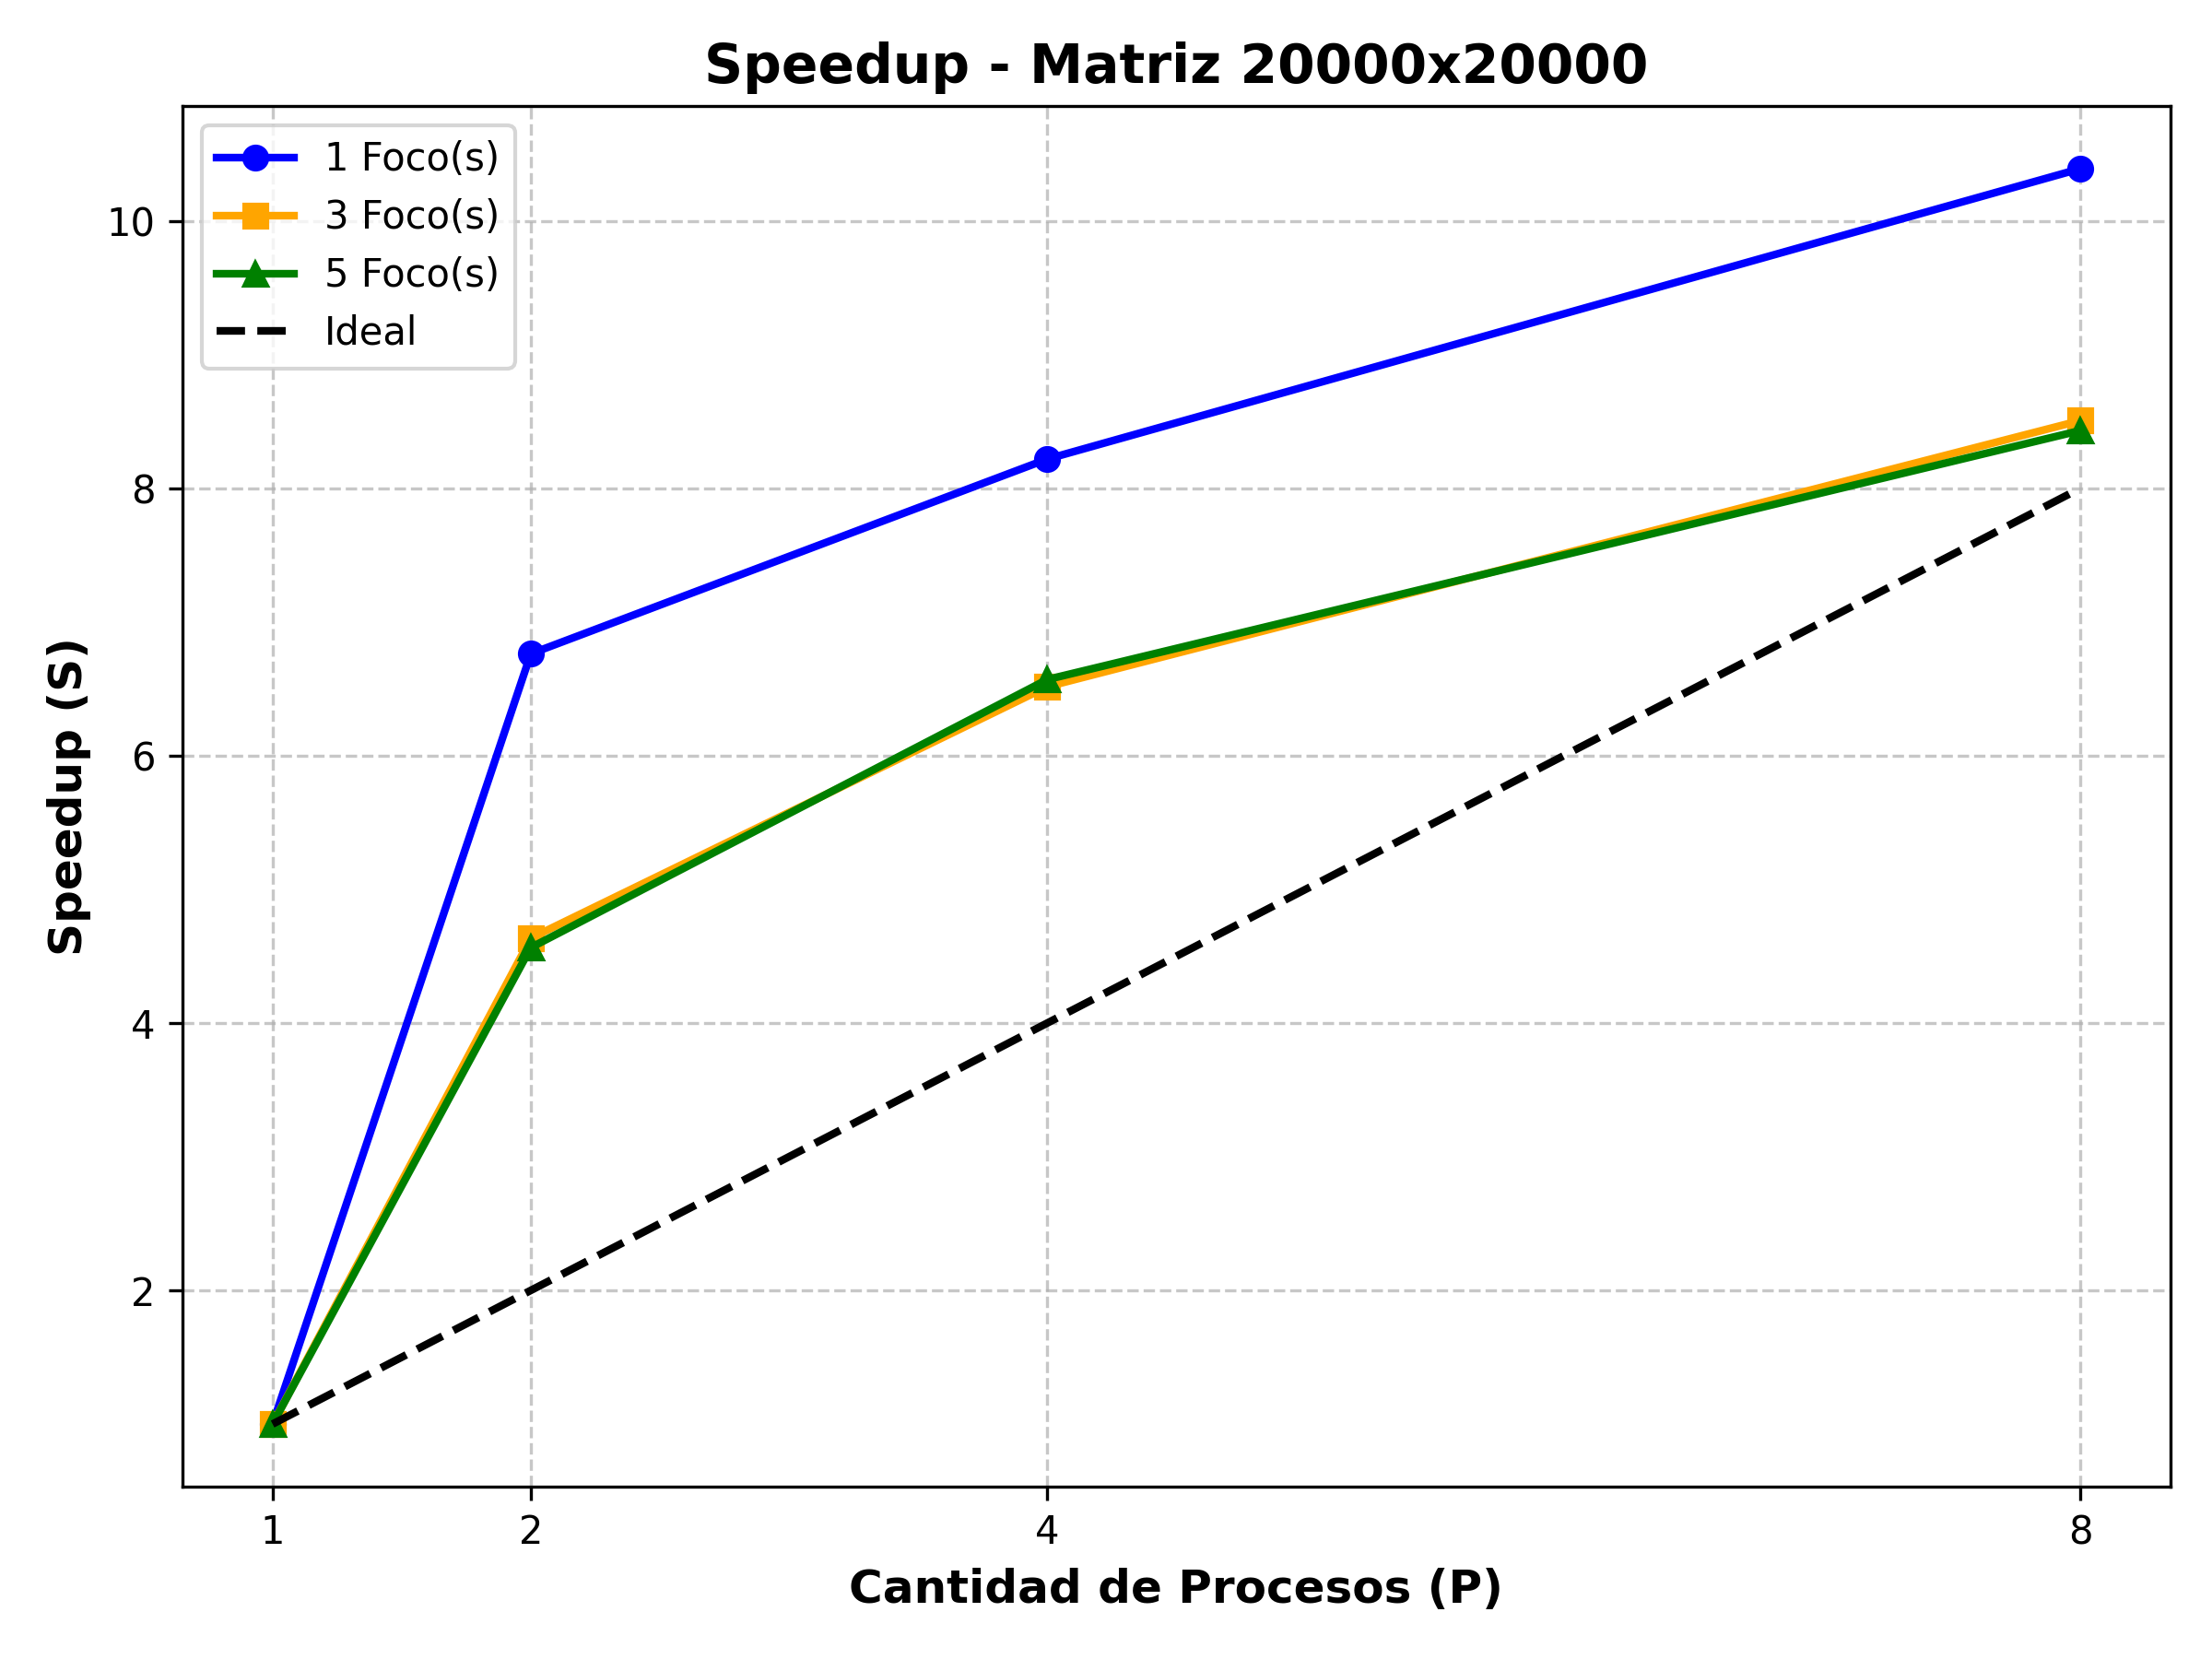
\includegraphics[width=0.32\textwidth]{graficos/speedup_20000x20000.png}
    \caption{Curvas de Speedup mostrando aceleración superlineal frente al límite teórico ideal.}
    \label{fig:speedup}
\end{figure}

\subsection{Eficiencia}
La métrica de Eficiencia se define clásicamente como $E = S / p$. En un escenario habitual, sus valores fluctúan entre $0$ y $1.0$ (o 0\% y 100\%). Sin embargo, dado que el sistema experimenta un pronunciado speedup superlineal a causa de la ganancia masiva de localidad de caché descrita en la sección anterior, el cálculo matemático arroja resultados mayores al 100\% (llegando a 130\% para $P=8$). Por este motivo, se ha decidido omitir la inclusión de gráficas de Eficiencia en este análisis, puesto que bajo estas condiciones de hardware, el valor numérico derivado ya no representa una medida fiable sobre el aprovechamiento intrínseco del paralelismo ni del \textit{overhead} de comunicación.

\subsection{Escalabilidad}
Más allá de la evidente reducción en los tiempos absolutos de ejecución, la escalabilidad del algoritmo queda demostrada por la solidez y persistencia de su comportamiento ante variaciones en la configuración experimental. La tendencia de aceleración superlineal no es un caso aislado, sino que se sostiene transversalmente al alterar tanto la carga dinámica de trabajo (1, 3 y 5 focos iniciales) como el tamaño estructural del dominio ($10000^2$, $15000^2$ y $20000^2$).

A pesar de esta tendencia sostenida, la escalabilidad encuentra su límite físico en la granularidad de la división y los tiempos de comunicación. Al realizar un \textit{profiling} interno detallado sobre la matriz de $10000^2$ con $P=8$ y 1 foco (Tabla \ref{tab:metricas_profiling}), se observa que el tiempo de cómputo útil promedio por iteración cae a $\sim0.31$ ms. Sin embargo, el tiempo de sincronización por red (\texttt{MPI\_Allreduce}) y el intercambio de halos (\texttt{MPI\_Sendrecv}) consumen en promedio $0.79$ ms. Esto demuestra concluyentemente por qué la curva de aceleración pierde pendiente en esta configuración: el volumen de cómputo por nodo es tan ínfimo que el \textit{overhead} de comunicación de la red domina la ejecución, representando casi el 70\% del tiempo de iteración. Por el contrario, en matrices de $20000^2$, el elevado volumen de cálculo local justifica ampliamente esta sobrecarga.


\subsection{Balanceo de carga}
A pesar de los excelentes números de rendimiento global, el algoritmo padece de un desbalance de carga inherente a la naturaleza espacial de un incendio. La Tabla \ref{tab:metricas_profiling} expone matemáticamente este fenómeno al comparar el trabajo realizado por cada uno de los 8 procesos de manera simultánea.

Al repartir la matriz de manera estática y simétrica, procesos como el \textit{Rank 3} concentran la mayor densidad de celdas en fuego (evaluando 1865 candidatos por iteración y demorando 0.376 ms en su fase de cómputo). En contraposición, procesos periféricos como el \textit{Rank 5} manejan apenas 1126 candidatos (consumiendo 0.253 ms). Dado que todos los procesos deben sincronizarse de forma bloqueante al final del bucle mediante el \texttt{MPI\_Allreduce} para determinar el corte global, los procesos más "descargados" deben aguardar inactivos en la barrera. Los datos empíricos lo confirman: el \textit{Rank 5} desperdicia 0.810 ms inactivo en la reducción, mientras que el \textit{Rank 3} solo espera 0.671 ms. Este desbalance de carga del 21.8\% entre el bloque más pesado y la media demuestra que el tiempo de ejecución global se ve íntegramente dictado por el proceso más sobrecargado, forzando al resto a desperdiciar valiosos ciclos de cómputo inactivos frente a la red.

% --- CONCLUSIÓN ---
\section{Conclusión}
El presente trabajo culminó con éxito en el diseño, implementación y evaluación empírica de un simulador distribuido de propagación de incendios forestales, combinando autómatas celulares con generación procedural de terrenos. La migración del algoritmo secuencial hacia una arquitectura de paso de mensajes utilizando MPI permitió superar de forma contundente las limitaciones de cómputo y memoria impuestas por la simulación de ecosistemas a gran escala.

El análisis exhaustivo de rendimiento destacó la obtención sostenida de un \textbf{speedup superlineal}. Este fenómeno demostró empíricamente cómo la partición espacial del dominio global masivo ($20000^2$ celdas) minimiza los fallos de caché (\textit{cache misses}), permitiendo que cada sub-bloque procesado resida eficientemente en la jerarquía de memoria (L2/L3) de cada nodo. Esta ganancia arquitectónica por localidad de datos resultó ser tan profunda que eclipsó el \textit{overhead} natural de comunicación de red introducido por MPI.

Por otro lado, el perfilado algorítmico permitió comprender a bajo nivel los límites físicos de escalabilidad y el comportamiento del sistema frente al desbalance de carga inherente a un fenómeno localizado como el fuego. Se comprobó matemáticamente cómo la división estática del mapa penaliza el tiempo global debido a las barreras de sincronización (\texttt{MPI\_Allreduce}), obligando a los procesos periféricos a desperdiciar ciclos de reloj inactivos mientras aguardan a los procesos centrales más sobrecargados.

En definitiva, la solución paralela desarrollada probó ser sumamente veloz y elástica (\textit{weak scaling}), reduciendo simulaciones que demandaban más de 12 minutos a apenas 1 minuto de reloj.

\subsection{Posibles mejoras}
A partir del análisis de rendimiento y las limitaciones observadas (fundamentalmente el desbalance de carga), se identifican dos líneas de mejora arquitectónica con distinto nivel de complejidad para optimizar aún más el simulador.

\textbf{1. Procesamiento por bloques activos.} Una primera mejora de complejidad moderada consiste en evitar que todos los procesos realicen el cómputo y comunicación de sus bloques completos en cada iteración. Para esto, se podría etiquetar un bloque como \textit{activo} únicamente si cumple al menos una de las siguientes condiciones:
\begin{itemize}
    \item Contiene fuego vivo localmente.
    \item Recibió fuego desde un bloque vecino mediante el intercambio de halos.
    \item Es adyacente a un bloque activo.
\end{itemize}
Con esta estrategia, los nodos alejados del frente del incendio podrían omitir el recorrido de sus celdas o permanecer inactivos, algo especialmente crítico en incendios altamente focalizados. Su implementación es accesible dado que conserva la división estática de la grilla, requiriendo apenas una comunicación marginal para propagar el estado.

\textbf{2. Balanceo de carga dinámico.} Como mejora avanzada, se propone abandonar la descomposición estática rígida en favor de una división hiper-granular (bloques mucho más pequeños). En este enfoque, los bloques activos podrían reasignarse dinámicamente entre los \textit{ranks} según la carga real de cada iteración. De esta manera, si un incendio se concentra en una zona del mapa, los recursos de todo el cluster podrían movilizarse allí, logrando un aprovechamiento óptimo. No obstante, esta mejora acarrea una alta complejidad algorítmica, exigiendo administrar colas de trabajo, migrar bloques en tiempo de ejecución y garantizar la coherencia de los halos en fronteras mutables.

% --- REFERENCIAS ---
\vspace{1cm}
\noindent \textbf{\fontsize{14}{17}\selectfont Referencias}
\begin{description}
    \item[{[Wol83]}] Wolfram, S.: Statistical mechanics of cellular automata. Reviews of Modern Physics 55(3), 1983
    \item[{[Gar70]}] Gardner, M.: Mathematical Games -- The fantastic combinations of John Conway's new solitaire game ``Life''. Scientific American 223(4), 1970
    \item[{[Per85]}] Perlin, K.: An image synthesizer. ACM SIGGRAPH Computer Graphics 19(3), 1985
    \item[{[EMP+03]}] Ebert, D. S.; Musgrave, F. K.; Peachey, D.; Perlin, K.; Worley, S.: Texturing \& Modeling: A Procedural Approach. 3rd ed. Morgan Kaufmann, 2003
    \item[{[Dur64]}] Durstenfeld, R.: Algorithm 235: Random permutation. Communications of the ACM 7(7), 1964
    \item[{[Ste14]}] Steele, G. L.; Lea, D.; Flood, C. H.: Fast splittable pseudorandom number generators. ACM SIGPLAN Notices 49(10), 2014
    \item[{[Cat24]}] Cátedra de Programación Paralela y Distribuida: Información, pautas y métricas provistas por la cátedra para el desarrollo y evaluación del proyecto. 2026
\end{description}

\end{document}